\chapter{Creating the Distributed Databases}\label{cha:Creating-Distributed-Databases}

After using \texttt{xmeshfem3D} or \texttt{xdecompose\_mesh}, the
next step in the workflow is to compile \texttt{xgenerate\_}~\newline
 \texttt{databases}. This program is going to create all the missing
information needed by the SEM solver.

\begin{figure}[htbp]
\begin{centering}
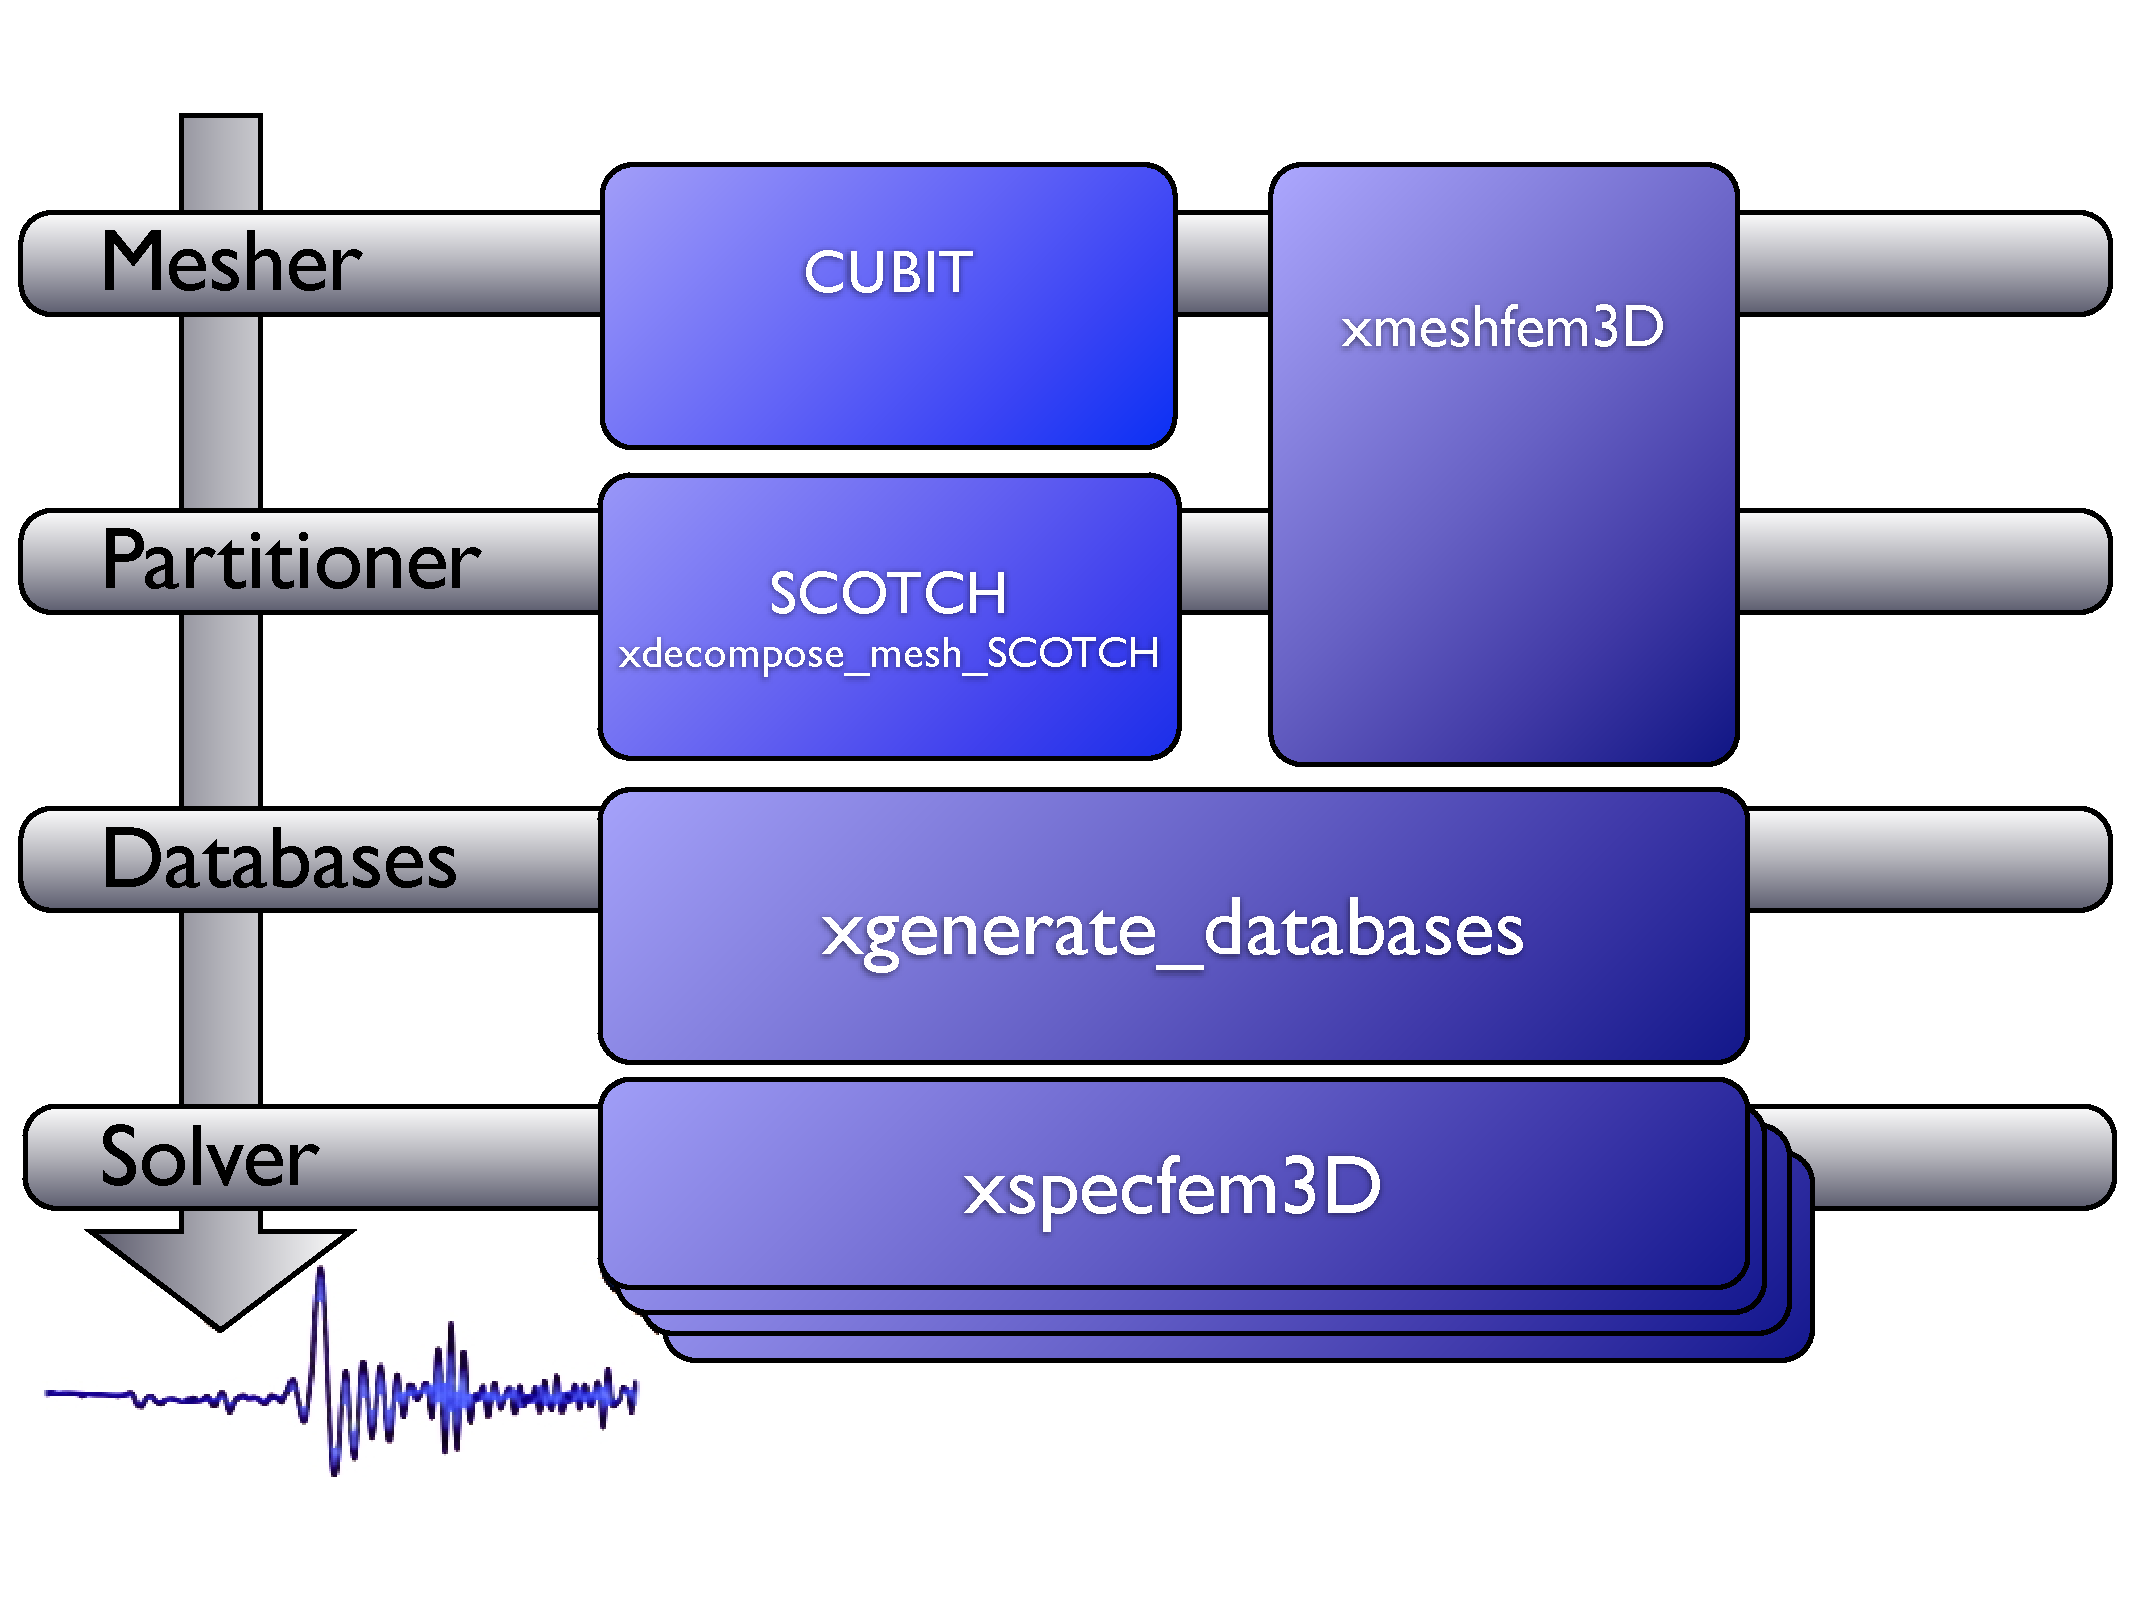
\includegraphics[width=0.6\textwidth]{figures/workflow.jpg}
\par
\end{centering}
\caption{Schematic workflow for a SPECFEM3D Cartesian simulation. The executable
\texttt{xgenerate\_databases} creates the GLL mesh points and assigns
specific model parameters.}
\label{fig:workflow.databases}
\end{figure}

\noindent
In the main directory, type
{\small
\begin{verbatim}
  make xgenerate_databases
\end{verbatim}
}
\noindent
Input for the program is provided through the main parameter file
\texttt{Par\_file}, which resides in the subdirectory \texttt{DATA}.
Please note that \texttt{xgenerate\_databases} must be called directly
from the main directory, as most of the binaries of the package.

\newpage
\section{Main parameter file \texttt{Par\_file}}\label{cha:Main-Parameter}

Before running \texttt{xgenerate\_databases}, a number of parameters
need to be set in the main parameter \texttt{Par\_file} located in
the subdirectory \texttt{DATA}:\newline

\noindent {\bf $\bullet$ Simulation setup}
\begin{description}
\item [{\texttt{SIMULATION\_TYPE}}] is set to 1 for forward simulations,
2 for adjoint simulations (see Section \ref{sec:Adjoint-simulation-finite})
and 3 for kernel simulations (see Section \ref{sec:Finite-Frequency-Kernels}).
\item [{\texttt{SAVE\_FORWARD}}] is only set to \texttt{.true.} for a forward
simulation with the last frame of the simulation saved, as part of
the finite-frequency kernel calculations (see Section \ref{sec:Finite-Frequency-Kernels}).
For a regular forward simulation, leave \texttt{SIMULATION\_TYPE}
and \texttt{SAVE\_FORWARD} at their default values.
\item [{\texttt{UTM\_PROJECTION\_ZONE}}] UTM projection zone in
which your model resides, only valid when \texttt{SUPPRESS\_UTM\_PROJECTION} is \texttt{.false.}.
\item [{\texttt{SUPPRESS\_UTM\_PROJECTION}}] set to be \texttt{.false.}
when your model range is specified in the geographical coordinates,
and needs to be \texttt{.true.} when your model is specified in a
cartesian coordinates. \noun{UTM projection zone in which your simulation
region resides.}
\item [{\texttt{NPROC}}] The number of MPI processors, each one is assigned
one slice of the whole mesh.
\item [{\texttt{NSTEP}}] The number of time steps of the simulation. This
controls the length of the numerical simulation, i.e., twice the number
of time steps requires twice as much CPU time. This feature is not
used at the time of generating the distributed databases but is required
for the solver, i.e., you may change this parameter after running
\texttt{xgenerate\_databases}.
\item [{\texttt{DT}}] The length of each time step in seconds. This feature
is not used at the time of generating the distributed databases but
is required for the solver. Please see also Section~\ref{sec:Choosing-the-Time-Step}
for further details.
\end{description}

\vspace{1cm}
\noindent {\bf $\bullet$ Mesh setup}
\begin{description}
\item [{\texttt{NGNOD}}] The number of nodes for 2D and 3D shape functions
for hexahedra. We use either 8-node mesh elements (bricks) or 27-node
elements. If you use the internal mesher, the only option is 8-node
bricks (27-node elements are not supported). \texttt{CUBIT} does not
support HEX27 elements either (it can generate them, but they are
flat, i.e. identical to HEX8). To generate HEX27 elements with curvature
properly taken into account, you can use Gmsh \url{http://gmsh.info}
\item [{\texttt{MODEL}}] Must be set to one of the following:

\begin{description}
\item [{\textmd{Models defined by mesh parameters:}}] ~

\begin{description}
\item [{\texttt{default}}] Uses model parameters as defined by meshing
procedures described in the previous Chapter~\ref{cha:Mesh-Generation}.
\end{description}

\item [{\textmd{1D~models~with~real~structure:}}] ~

\begin{description}
\item [{\texttt{1D\_prem}}] Isotropic version of the spherically symmetric
Preliminary Reference Earth Model (PREM) \citep{DzAn81}.
\item [{\texttt{1D\_socal}}] A standard isotropic 1D model for Southern
California.
\item [{\texttt{1D\_cascadia}}] Isotropic 1D profile for the Cascadia region.
\end{description}

\item [{\textmd{Fully~3D~models:}}] ~

\begin{description}
\item [{\texttt{aniso}}] For a user-specified fully anisotropic model.
Parameters are set up in routines located in file \texttt{model\_aniso.f90}
in directory \texttt{src/generate\_databases/}. See Chapter~\ref{cha:-Changing-the}
for a discussion on how to specify your own 3D model.

\item [{\texttt{external}}] For a user-specified isotropic model which
uses externally defined model parameters. Uses external model definitions
set up in routines located in file \texttt{model\_external\_values.f90}
in directory \texttt{src/generate\_databases/}. Please modify these
generic template routines to use your own model definitions.

\item [{\texttt{gll}}] For a user-specified isotropic model which uses
external binary files for $v_{p}$, $v_{s}$ and $\rho$. Binary files
are given in the same format as when outputted by the \texttt{xgenerate\_databases}
executable when using option \texttt{SAVE\_MESH\_FILES}. These binary
files define the model parameters on all GLL points which can be used
for iterative inversion procedures. Note that for simulation setups with attenuation,
it will also read in the external binary mesh files for $Q_{\kappa}$ and $Q_{\mu}$.
Note that Qmu is always equal to Qs, but Qkappa is in general not equal to Qp.
To convert one to the other see \texttt{doc/note\_on\_Qkappa\_versus\_Qp.pdf}
and in folder \texttt{utils/attenuation}, the tool
\texttt{conversion\_from\_Qkappa\_Qmu\_to\_Qp\_Qs\_from\_Dahlen\_Tromp\_959\_960.f90}.


\item [{\texttt{salton\_trough}}] A 3D $V_{p}$ model for Southern California.
Users must provide the corresponding data file \texttt{regrid3\_vel\_p.bin}
in directory \texttt{DATA/st\_3D\_block\_harvard/}.

\item [{\texttt{tomo}}] For a user-specified 3D isotropic model which uses
a tomographic model file \texttt{tomography\_model.xyz} in directory
\texttt{DATA}. See Section \ref{sec:Using-tomographic}, for a discussion
on how to specify your own 3D tomographic model.
\end{description}
\end{description}

\item [{\texttt{APPROXIMATE\_OCEAN\_LOAD}}] Set to \texttt{.true.} if the
effect of the oceans on seismic wave propagation should be incorporated
based upon the (rough) approximate treatment discussed in \citet{KoTr02b}.
This feature is inexpensive from a numerical perspective, both in
terms of memory requirements and CPU time. This approximation is accurate
at periods of roughly 20~s and longer. At shorter periods the effect
of water phases/reverberations is not taken into account, even when
the flag is on. If you want to model the effect of a fluid-solid model
at short periods, then set this flag to \texttt{.false.} and mesh
the fluid layer explicitly in your mesher, so that it is computed
accurately and without this approximation.
\item [{\texttt{TOPOGRAPHY}}] This feature is only effective if \texttt{APPROXIMATE\_OCEAN\_LOAD}
is set to \texttt{.true.}. Set to \texttt{.true.} if topography and
bathymetry should be read in based upon the topography file specified
in the main constants file \texttt{setup/constants.h} to evaluate elevations. If not set, elevations
will be read from the numerical mesh.
\item [{\texttt{ATTENUATION}}] Set to \texttt{.true.} if attenuation should
be incorporated. Turning this feature on increases the memory requirements
significantly (roughly by a factor of~1.5), and is numerically fairly
expensive. See \citet{KoTr99,KoTr02a} for a discussion on the implementation
of attenuation based upon standard linear solids. Please note that
the Vp- and Vs-velocities of your model are given for a reference
frequency. To change this reference frequency, you change the value
of \texttt{ATTENUATION\_f0\_REFERENCE} defined (in Hz) in input file \texttt{DATA/Par\_file}.
The code uses a constant $Q$ quality factor, write(IMAIN,*) "but approximated based on a series of Zener standard linear solids (SLS).
The approximation is thus performed in a given frequency band determined based on that \texttt{ATTENUATION\_f0\_REFERENCE} reference frequency.
Note that Qmu is always equal to Qs, but Qkappa is in general not equal to Qp.
To convert one to the other see \texttt{doc/note\_on\_Qkappa\_versus\_Qp.pdf}
and in folder \texttt{utils/attenuation}, the tool
\texttt{conversion\_from\_Qkappa\_Qmu\_to\_Qp\_Qs\_from\_Dahlen\_Tromp\_959\_960.f90}.

\item [{\texttt{ANISOTROPY}}] Set to \texttt{.true.} if you want to use
an anisotropy model. Please see the file \texttt{model\_aniso.f90}
in subdirectory \texttt{src/generate\_databases/} for the current
implementation of anisotropic models.
\item [{\texttt{TOMOGRAPHY\_PATH}}] Directory in which the tomography files
are stored for using external tomographic Earth models (please read
Chapter \ref{cha:-Changing-the} and Section \ref{sec:Using-tomographic}
`Using external tomographic Earth models' for further details.).
\item [{\texttt{USE\_OLSEN\_ATTENUATION}}] Set to \texttt{.true.} if you
want to use the attenuation model that scaled from the S-wave speed
model using Olsen's empirical relation (see \citet{OlDaBr03}).
\item [{\texttt{OLSEN\_ATTENUATION\_RATIO}}] Determines the Olsen's constant
in Olsen's empirical relation (see \citet{OlDaBr03}).
\end{description}

\vspace{1cm}
\noindent {\bf $\bullet$ Absorbing boundary conditions setup}
\begin{description}
\item [{\texttt{PML\_CONDITIONS}}] Set to \texttt{.true.} to turn on C-PML
boundary conditions for a regional simulation. Both fluids and elastic solids are supported.
\item [{\texttt{PML\_INSTEAD\_OF\_FREE\_SURFACE}}] Set to \texttt{.true.}
to turn on C-PML boundary conditions on the top surface instead of
the usual free surface.
\item [{\texttt{f0\_FOR\_PML}}] Determines the dominant frequency that
will be used in the calculation of PML damping profiles;
\red{This should be set to the same (or similar) dominant frequency as that of the
source that you will use in your simulation. It is \textbf{VERY IMPORTANT} to do that, otherwise the PML
absorbing conditions can become unstable.}
If you plan to use a Dirac source, then use the dominant frequency of the source wavelet
with which you plan to convolve your seismograms later on in post-processing.
\item [{\texttt{STACEY\_ABSORBING\_CONDITIONS}}] Set to \texttt{.true.}
to turn on Clayton-Engquist absorbing boundary conditions (see \citet{KoTr99}).
In almost all cases it is much better to use CPML absorbing layers
(see the options above) and leave this flag to \texttt{.false.}.
\item [{\texttt{STACEY\_INSTEAD\_OF\_FREE\_SURFACE}}] Set to \texttt{.true.}
to turn on absorbing boundary conditions on the top surface which
by default constitutes a free surface of the model.
\item [{\texttt{BOTTOM\_FREE\_SURFACE}}]
When STACEY\_ABSORBING\_CONDITIONS is set to .true. :
absorbing conditions are defined in xmin, xmax, ymin, ymax and zmin
this option BOTTOM\_FREE\_SURFACE can be set to .true. to
make zmin free surface instead of absorbing condition.
\end{description}

\vspace{1cm}
\noindent {\bf $\bullet$ Visualization setup}
\begin{description}
\item [{\texttt{CREATE\_SHAKEMAP}}] Set this flag to \texttt{.true.} to
create a ShakeMap\textregistered{}, e.g., a peak ground velocity map
of the maximum absolute value of the two horizontal components of
the velocity vector.
\item [{\texttt{MOVIE\_SURFACE}}] Set to \texttt{.false.}, unless you want
to create a movie of seismic wave propagation on the Earth's surface.
Turning this option on generates large output files. See Section~\ref{sec:Movies}
for a discussion on the generation of movies. This feature is only
relevant for the solver.
\item [{\texttt{MOVIE\_TYPE}}] Set this flag to 1 to show the top surface
(tomography + oceans) only, to 2 to show all external faces of the
mesh (i.e. topography + vertical edges + bottom) in shakemaps and
surface movies.
\item [{\texttt{MOVIE\_VOLUME}}] Set to \texttt{.false.}, unless you want
to create a movie of seismic wave propagation in the Earth's interior.
Turning this option on generates huge output files. See Section~\ref{sec:Movies}
for a discussion on the generation of movies. This feature is only
relevant for the solver.
\item [{\texttt{SAVE\_DISPLACEMENT}}] Set this flag to \texttt{.true.}
if you want to save the displacement instead of velocity for the movie
frames.
\item [{\texttt{USE\_HIGHRES\_FOR\_MOVIES}}] Set this flag to \texttt{.true.}
if you want to save the values at all the NGLL grid points for the
movie frames.
\item [{\texttt{NTSTEP\_BETWEEN\_FRAMES}}] Determines the number of timesteps
between movie frames. Typically you want to save a snapshot every
100 timesteps. The smaller you make this number the more output will
be generated! See Section~\ref{sec:Movies} for a discussion on the
generation of movies. This feature is only relevant for the solver.
\item [{\texttt{HDUR\_MOVIE}}] Determines the half duration of the source
time function for the movie simulations. When this parameter is set
to be 0, a default half duration that corresponds to the accuracy
of the simulation is provided. Otherwise, it adds this half duration
to the half duration specified in the source file \texttt{CMTSOLUTION},
thus simulates longer periods to make the movie images look smoother.
\item [{\texttt{SAVE\_MESH\_FILES}}] Set this flag to \texttt{.true.} to
save \href{www.paraview.org}{ParaView} mesh files for
subsequent viewing. Turning the flag on generates large (distributed)
files in the \texttt{LOCAL\_PATH} directory. See Section~\ref{sec:Mesh-graphics}
for a discussion of mesh viewing features.
\item [{\texttt{LOCAL\_PATH}}] Directory in which the distributed databases
will be written. Generally one uses a directory on the local disk
of the compute nodes, although on some machines these databases are
written on a parallel (global) file system (see also the earlier discussion
of the \texttt{LOCAL\_PATH\_IS\_ALSO\_GLOBAL} flag in Chapter~\ref{cha:Getting-Started}).
\texttt{xgenerate\_databases} generates the necessary databases in
parallel, one set for each of the \texttt{NPROC} slices that constitutes
the mesh (see Figure~\ref{fig:mount.partitions} and Figure~\ref{fig:For-parallel-computing}).
After the executable finishes, you can log in to one of the compute
nodes and view the contents of the \texttt{LOCAL\_PATH} directory
to see the (many) files generated by \texttt{xgenerate\_databases}.
Please note that the \texttt{LOCAL\_PATH} directory should already
contain the output files of the partitioner, i.e. from \texttt{xdecompose\_mesh}
or \texttt{xmeshfem3D}.
\item [{\texttt{NTSTEP\_BETWEEN\_OUTPUT\_INFO}}] This parameter specifies
the interval at which basic information about a run is written to
the file system (\texttt{timestamp{*}} files in the \texttt{OUTPUT\_FILES}
directory). If you have access to a fast machine, set \texttt{NTSTEP\_BETWEEN\_OUTPUT\_INFO}
to a relatively high value (e.g., at least 100, or even 1000 or more)
to avoid writing output text files too often. This feature is not
used at the time of meshing. One can set this parameter to a larger
value than the number of time steps to avoid writing output during
the run.
\end{description}

\vspace{1cm}
\noindent {\bf $\bullet$ Sources setup}
\begin{description}
\item [{\texttt{USE\_FORCE\_POINT\_SOURCE}}] Turn this flag on to use a
(tilted) \texttt{FORCESOLUTION} force point source instead of a \texttt{CMTSOLUTION}
moment-tensor source. When the force source does not fall exactly
at a grid point, the solver interpolates the force between grid points
using Lagrange interpolants. This can be useful e.g. for oil industry
foothills simulations in which the source is a vertical force, normal
force, tilted force, or an impact etc. Note that in the \texttt{FORCESOLUTION}
file, you will need to edit the East, North and vertical components
of an arbitrary (not necessarily unitary, the code will normalize it automatically) direction vector of the force vector;
thus refer to Appendix~\ref{cha:Coordinates} for the orientation
of the reference frame. This vector is made unitary internally in
the solver and thus only its direction matters here; its norm is ignored
and the norm of the force used is the factor force source times the
source-time function.

When using this option, by default the code can locate the force source
anywhere between mesh points in order to honor its exact location; this
is more precise than using the closest GLL mesh point, but it is also a bit slower.
\item [{\texttt{USE\_RICKER\_TIME\_FUNCTION}}] Turn this flag on to use
a Ricker source-time function, i.e., the second derivative of a Gaussian, instead of the source-time functions
set by default to represent a (tilted) \texttt{FORCESOLUTION} force
point source or a \texttt{CMTSOLUTION} moment-tensor source.
Note that we use the standard definition of a Ricker, for a dominant frequency $f_0$:
$\mathrm{Ricker}(t) = (1 - 2 a t^2) e^{-a t^2}$, with $a = \pi^2 f_0^2$,
whose Fourier transform is thus:
$\frac{1}{2} \frac{\sqrt{\pi}\omega^2}{a^{3/2}}e^{-\frac{\omega^2}{4 a}}$
This gives the wavelet of Figure~\ref{fig:RickerWavelet}.
%%
\begin{figure}[htbp]
\centering
\includegraphics[width=3in]{figures/Ricker_wavelet.png}
\caption{We use the standard definition of a Ricker (i.e., second derivative of a Gaussian). Image taken from \url{http://subsurfwiki.org}.}
\label{fig:RickerWavelet}
\end{figure}
%%
Originally, if a \texttt{CMTSOLUTION} moment-tensor source is used, a (pseudo)
Heaviside step function with a very short half duration is defined
for elastic cases to represent the permanent slip on the fault while
in the acoustic case a Gaussian source-time function with a similarly
short half duration is defined to physically describe actions within
the fluid. Otherwise, if a \texttt{FORCESOLUTION} force source is
used, a (pseudo) Dirac delta source-time function is defined by default.
Any other source-time function may then be obtained by convolution.
\item [{\texttt{PRINT\_SOURCE\_TIME\_FUNCTION}}] Turn this flag on to print
information about the source-time function in the file \texttt{OUTPUT\_FILES/plot\_source\_time\_function.txt}.
This feature is only relevant for the solver.
%
\end{description}

\vspace{1cm}
\noindent {\bf $\bullet$ Additionals}
\begin{description}
\item [{\texttt{NTSTEP\_BETWEEN\_OUTPUT\_SEISMOS}}] This parameter specifies
the interval at which synthetic seismograms are written in the \texttt{LOCAL\_PATH}
directory. If a run crashes, you may still find usable (but shorter
than requested) seismograms in this directory. On a fast machine set
\texttt{NTSTEP\_BETWEEN\_OUTPUT\_SEISMOS} to a relatively high value
to avoid writing to the seismograms too often. This feature is only
relevant for the solver.

\item [{\texttt{NUMBER\_OF\_SIMULTANEOUS\_RUNS}}] adds the ability to run several calculations (several earthquakes)
in an embarrassingly-parallel fashion from within the same run;
this can be useful when using a very large supercomputer to compute
many earthquakes in a catalog, in which case it can be better from
a batch job submission point of view to start fewer and much larger jobs,
each of them computing several earthquakes in parallel.

To turn that option on, set parameter \texttt{NUMBER\_OF\_SIMULTANEOUS\_RUNS} to a value greater than 1.
To implement that, we create \texttt{NUMBER\_OF\_SIMULTANEOUS\_RUNS} MPI sub-communicators,
each of them being labeled \texttt{my\_local\_mpi\_comm\_world}, and we use them
in all the routines in "src/shared/parallel.f90", except in MPI\_ABORT() because in that case
we need to kill the entire run.

When that option is on, of course the number of processor cores used to start
the code in the batch system must be a multiple of \texttt{NUMBER\_OF\_SIMULTANEOUS\_RUNS},
all the individual runs must use the same number of processor cores,
which as usual is NPROC in the \texttt{DATA/Par\_file},
and thus the total number of processor cores to request from the batch system
should be \texttt{NUMBER\_OF\_SIMULTANEOUS\_RUNS}~*~\texttt{NPROC}.
All the runs to perform must be placed in directories called run0001, run0002, run0003 and so on
(with exactly four digits).\newline

Imagine you have 10 independent calculations to do, each of them on 100 cores; you have three options:\newline

1/ submit 10 jobs to the batch system\newline

2/ submit a single job on 1000 cores to the batch, and in that script create a sub-array of jobs to start 10 jobs,
each running on 100 cores (see e.g. \url{http://www.schedmd.com/slurmdocs/job_array.html})\newline

3/ submit a single job on 1000 cores to the batch, start SPECFEM3D on 1000 cores, create 10 sub-communicators,
cd into one of 10 subdirectories (called e.g. run0001, run0002,... run0010) depending on the sub-communicator
your MPI rank belongs to, and run normally on 100 cores using that sub-communicator.\newline

The option \texttt{NUMBER\_OF\_SIMULTANEOUS\_RUNS} implements 3/.\newline

\item [{\texttt{BROADCAST\_SAME\_MESH\_AND\_MODEL}}] if we perform simultaneous runs in parallel,
if only the source and receivers vary between these runs
but not the mesh nor the model (velocity and density) then we can also read the mesh and model files
from a single run in the beginning and broadcast them to all the others; for a large number of simultaneous
runs for instance when solving inverse problems iteratively this can DRASTICALLY reduce I/Os to disk in the solver
(by a factor equal to \texttt{NUMBER\_OF\_SIMULTANEOUS\_RUNS}), and reducing I/Os is crucial in the case of huge runs.
Thus, always set this option to .true. if the mesh and the model are the same for all simultaneous runs.
In that case there is no need to duplicate the mesh and model file database (the content of the DATABASES\_MPI
directories) in each of the run0001, run0002,... directories, it is sufficient to have one in run0001
and the code will broadcast it to the others).\newline

%\item [{\texttt{USE\_FAILSAFE\_MECHANISM}}] if one or a few of these simultaneous runs fail,
%kill all the runs or let the others finish using a fail-safe mechanism
%(in most cases, should be set to true).

TODO / future work to do: currently the \texttt{BROADCAST\_SAME\_MESH\_AND\_MODEL}
option assumes to have the (main) mesh files in \texttt{run0001/DATABASES\_MPI} or
\texttt{run0001/OUTPUT\_FILES/DATABASES\_MPI}.
However, for adjoint runs you still need a \texttt{DATABASES\_MPI/} folder in each of the sub-runs directories,
e.g. \texttt{run0002/DATABASES\_MPI}, etc. to store the forward wavefields, kernels etc. of each sub-run.
This would not be needed for forward simulations.\newline

TODO / future work to do: the sensitivity kernel summing and smoothing tools in directory src/tomography are currently not ported to this new option to do many runs simultaneously, only the solver (src/specfem3d) is. Thus these tools should work, but in their current version will need to be run for each simulation result independently.\newline

More precisely, the current kernel summing and smoothing routines work fine, with the exception that you need to move out the mesh files (and also the parameters). This works because these routines consider multiple runs by design. You simply have to provide them the directories where the kernels are.\newline

\item [{\texttt{GPU\_MODE}}] Turn this flag on to use GPUs.

\item [\texttt{ADIOS\_ENABLED}] Turn this flag on to enable ADIOS. If set to \texttt{.false.}, subsequent ADIOS
parameters will not be considered.
\item [\texttt{ADIOS\_FOR\_DATABASES}] Turn this flag on to use ADIOS for xmeshfem3D output and
xgenerate\_database input.
\item [\texttt{ADIOS\_FOR\_MESH}]  Turn this flag on to use ADIOS for generated databases.
\item [\texttt{ADIOS\_FOR\_FORWARD\_ARRAYS}] Turn this flag on to read and write forward arrays using ADIOS.
\item [\texttt{ADIOS\_FOR\_KERNELS}] Turn this flag on to produce ADIOS kernels that can later be visualized with the ADIOS version of combine\_vol\_data.
\end{description}
There are quite a few more parameters to change the default setup of your runs. Please check the comments in the \texttt{DATA/Par\_file} directly for further explanations.\newline


\subsection{PML absorbing boundary layers}

If you use PML, the mesh elements that belong to the PML layers can
be acoustic or elastic, but not viscoelastic nor poroelastic. Then,
when defining your model, you should define these absorbing elements
as either acoustic or elastic. In you forget to do that, the code
will fix the problem by automatically converting the viscoelastic
or poroelastic PML elements to elastic. This means that strictly speaking
the PML layer will not be perfectly matched any more, since the physical
model will change from viscoelastic or poroelastic to elastic at the
entrance of the PML, but in practice this is sufficient and produces
only tiny / negligible spurious reflections.\newline


If you use PML and an external mesh (created using an external meshing tool
such as CUBIT/TRELIS or similar), try to have elements inside the PML as regular as possible,
i.e. ideally non-deformed cubes obtained by `extrusion' of regular surface mesh elements meshing the
outer edges of the computational domain without PML; by doing so, the PMLs obtained will be far more stable
in time (PML being weakly unstable from a mathematical point of view, very deformed mesh elements
inside the PMLs can trigger instabilities much more quickly). \red{We have two utilities in directory utils/CPML that do that automatically
and that are very fast}. To stabilize PMLs it also helps to add a transition layer of geometrically-regular non-PML elements, in which attenuation is also
turned off (i.e. $Q_\kappa = Q_\mu = 9999$ in that layer), as in the red layer of Figure~\ref{fig:mesh_extrusion}.
Our tools in directory utils/CPML implement that transition layer automatically.\newline


If you use PML and an external tomographic velocity and density model,
you should be careful because mathematically a PML cannot handle heterogeneities
along the normal to the PML edge inside the PML layer. This comes
from the fact that the damping profile that is defined assumes a constant
velocity and density model along the normal direction.
Thus, you need to modify your velocity and density model in order
for it to be 1D inside the PML, as shown in Figure~\ref{fig:modify_external_velocity_model_to_use_PML}.
This applies to the bottom layer as well; there you should make sure
that your model is 1D and thus constant along the vertical direction.\newline


To summarize, only use a 3D velocity and density model inside the
physical region, and in all the PML layers extend it by continuity
from its values along the inner PML edge.\newline

%%
\begin{figure}[htbp]
\noindent \begin{centering}
\includegraphics[width=4.5in]{figures/how_to_use_a_transition_mesh_layer_to_stabilize_PML.png}
\par\end{centering}
\caption{Mesh extrusion for PML (green elements) and a non-PML stabilization layer (red elements).}
\label{fig:mesh_extrusion}
\end{figure}
%%

%%
\begin{figure}[htbp]
\noindent \begin{centering}
\includegraphics[width=6in]{figures/how_to_use_PML_when_a_tomographic_velocity_model_is_used.png}
\par\end{centering}
\caption{How to modify your external 3D velocity and density model in order
to use PML. Such a modification is not needed when using Stacey absorbing
boundary conditions (but such conditions are significantly less efficient).}
\label{fig:modify_external_velocity_model_to_use_PML}
\end{figure}
%%


\section{Choosing the time step \texttt{DT}}\label{sec:Choosing-the-Time-Step}

The parameter \texttt{DT} sets the length of each time step in seconds.
The value of this parameter is crucial for the stability of the spectral-element
simulation. Your time step \texttt{DT} will depend on the minimum
ratio between the distance $h$ of neighboring mesh points and the
wave speeds $v$ defined in your model. The condition for the time
step $\Delta t$ is:
\begin{lyxcode}
$\Delta t<C~\mathrm{min}_{\Omega}(~h/v~)$
\end{lyxcode}
where $C$ is the so-called Courant number and $\Omega$ denotes the
model volume. The distance $h$ depends on the mesh element size and
the number of GLL points \texttt{NGLL} specified in the main constants
file \texttt{setup/constants.h}. The wave speed $v$ is determined based on your model's P- (or S-)
wave speed values.\newline


The database generator \texttt{xgenerate\_databases}, as well as the
internal mesher \texttt{xmeshfem3D}, are trying to evaluate the value
of $\Delta t$ for empirically chosen Courant numbers $C\sim0.3$.
If you used the mesher \texttt{xmeshfem3D} to generate your mesh,
you should set the value suggested in \texttt{OUTPUT\_FILES/output\_mesher.txt}
file, which is created after the mesher completed. In case you used
CUBIT to create the mesh, you might use an arbitrary value when running
\texttt{xgenerate\_databases} and then use the value suggested in
the ~\newline
 \texttt{OUTPUT\_FILES/output\_mesher.txt} file after the database
generation completed. Note that the implemented Newmark time scheme
uses this time step globally, thus your simulations become more expensive
for very small mesh elements in high wave-speed regions. Please be
aware of this restriction when constructing your mesh in Chapter~\ref{cha:Mesh-Generation}.

